\chapter{波、相位与复振幅：干涉的最小语言}
\label{chap:e01}

\begin{chapteropening}
想象你站在一座望远镜的焦点后面，一束星光刚刚落进来。它在物理上是什么？是一段飞快摆动的电场——快到什么程度呢？一个来回只要几飞秒，比你眨一次眼快上万亿倍。可是当这束光最终变成数据时，那飞快的摆动却"消失"了，探测器只留下一个安静的数字：强度，或者说光子计数。摆动去哪了？相位又去哪了？

本章要做的事，就是把"波的语言"从最底层讲起：先写下一段单色电磁波，再学会用一支"旋转的箭头"（复振幅）同时装下它的振幅和相位；然后弄清楚探测器为什么只看得见振幅的平方、看不见相位本身；最后让两束光相遇，看干涉是怎么把"看不见的相位差"重新变成"看得见的亮暗"。这几件事，是后面所有相干、干涉、强度关联章节共同的字母表。
\end{chapteropening}

\section{单色电磁波：一段飞快摆动的电场}
\label{sec:e01-wave}

先把画面立起来。在一个足够窄的频率通道里，星光可以近似当成一列\textbf{单色光}（monochromatic light）：它只有一个频率，像一根纯音。真正在振荡的，是空间某一点上的电场强度——它随时间上上下下，像一根被拨动后稳定摆动的弦。数学上把它写成

\begin{equation}
  E(t)=E_0\cos(\omega t+\phi),\qquad \omega=2\pi\nu .
  \label{eq:e01-monochromatic}
\end{equation}
\begin{formulaexplain}
\(E(t)\) 是 \(t\) 时刻的电场；\(E_0\) 是振幅（摆动的最大幅度）；\(\omega\) 是角频率，\(\nu\) 是普通频率，二者相差一个 \(2\pi\)；\(\phi\) 是初相位，决定 \(t=0\) 时摆到了哪儿。
\end{formulaexplain}

逐个符号落地。\(E(t)\) 是电场，在 CGS 单位里量纲是 \({\rm statvolt\,cm^{-1}}\)，但对本章的推导来说，它具体多大并不重要，重要的是它\emph{怎样随时间变化}。\(E_0\) 是这段摆动的最大高度，也就是振幅（amplitude），它同样是电场的量纲。\(\phi\) 是初相位（phase），单位是弧度，是一个纯粹的角度、无量纲——你可以把它读成"在 \(t=0\) 这一刻，摆动进行到了周期里的哪个位置"。

括号里的 \(\omega t+\phi\) 整体叫\textbf{瞬时相位}（instantaneous phase）：随着时间流逝，\(\omega t\) 均匀增大，余弦就一遍遍地从 \(+1\) 荡到 \(-1\) 再荡回来。角频率 \(\omega\) 的单位是 \({\rm rad\,s^{-1}}\)，它告诉我们相位涨得多快；普通频率 \(\nu\)（单位 Hz，即每秒多少个整周期）与它的关系是 \(\omega=2\pi\nu\)，因为绕一整圈是 \(2\pi\) 弧度。周期是 \(T=1/\nu=2\pi/\omega\)。

现在代入真实数字，感受一下这有多快。可见光的频率大约在

\[
  \nu\simeq 4\times10^{14}\ {\rm Hz}\ (\text{红光})\quad\text{到}\quad 8\times10^{14}\ {\rm Hz}\ (\text{蓝光}),
\]

于是一个周期只有

\[
  T=\frac{1}{\nu}\simeq\frac{1}{5\times10^{14}\ {\rm Hz}}=2\times10^{-15}\ {\rm s}=2\ {\rm fs}.
\]

也就是说，可见光的电场每两飞秒就完成一次完整的上下摆动。飞秒（\(10^{-15}\) 秒）是什么概念？光在一飞秒里只跑 \(0.3\ \mu{\rm m}\)，还不到一根头发丝直径的百分之一。任何常规天文探测器——无论是 CCD 像素、光电倍增管还是雪崩二极管——它的响应时间至少是纳秒（\(10^{-9}\) 秒）量级，比一个光学周期慢了 \(10^{5}\)–\(10^{6}\) 倍（拿"至少 \(1\ {\rm ns}\)"去比"约 \(2\ {\rm fs}\)"，\(1\ {\rm ns}/2\ {\rm fs}\approx5\times10^{5}\)；若换成积分时间到微秒量级的 CCD，那就更慢）。

这就带来一个贯穿全书的关键事实：探测器"太慢"了，它根本跟不上电场逐周期的正负摆动。在探测器眨一次“电子学的眼”的时间里，电场已经上下荡了几十万乃至上百万个来回。它不可能把每一次摆动都记下来，只能把这些飞快的振荡在自己的响应时间里\emph{抹平}，最后留下一个平均能量。于是 \(E(t)\) 里那个飞快变化的、带着相位信息的部分，探测器\textbf{直接看不见}。我们后面会看到，正是这一点逼着人们去发明干涉与关联测量——那是把"看不见的相位"重新变回"看得见的强度"的唯一办法。

\section{复振幅：把振幅和相位装进一支旋转箭头}
\label{sec:e01-phasor}

式~\eqref{eq:e01-monochromatic} 有点笨重：每次讨论两束光相加、相位差怎么变，都要摆弄一堆余弦的和差化积公式。有没有更聪明的记法，能把\emph{振幅}和\emph{相位}这两件事一次装好、还让加法变简单？有，这就是\textbf{复振幅}（complex amplitude，也叫 phasor，相量）。

先给画面。把余弦想成一支从原点出发、绕着原点匀速旋转的箭头在水平轴上的投影：箭头的\emph{长度}就是振幅 \(E_0\)，箭头指向的\emph{角度}就是瞬时相位 \(\omega t+\phi\)。箭头以角速度 \(\omega\) 逆时针转\footnote{这里选了 \(e^{+i\omega t}\) 这一支时间约定：箭头逆时针旋转，正频率取 \(+i\omega t\)。本章之内它完全自洽，所有结论都不受影响。提醒一句以免日后对接时困惑：等到后面引入正/负频率场算符 \(\hat E^{(+)},\hat E^{(-)}\) 做二次量子化时，含湮灭算符 \(\hat a\) 的正频率部分 \(\hat E^{(+)}\) 通常按 \(e^{-i\omega t}\) 演化，箭头转向与这里相反。两种约定只是同一物理的镜像记法——把这里所有的 \(i\) 换成 \(-i\)（等价于把箭头看成顺时针转）即可平滑对接，物理内容一字不改。}，它在实轴（水平方向）上的影子，正好就是 \(E_0\cos(\omega t+\phi)\)。于是"一段振荡的场"被翻译成"一支旋转的箭头"。既然要描述平面上的箭头，用复数最自然——复平面上一个点，天生就带着"长度"和"角度"两个信息。

我们把箭头在 \(t=0\) 时刻的样子（长度 \(E_0\)、角度 \(\phi\)）打包成一个复数：

\begin{equation}
  \mathcal{E}=E_0e^{i\phi},\qquad E(t)=\operatorname{Re}\!\left[\mathcal{E}\,e^{i\omega t}\right].
  \label{eq:e01-phasor}
\end{equation}
\begin{formulaexplain}
\(\mathcal E\) 是复振幅；它的模 \(|\mathcal E|=E_0\) 是振幅，辐角 \(\arg\mathcal E=\phi\) 是相位。乘上旋转因子 \(e^{i\omega t}\) 让箭头转起来，再取实部 \(\operatorname{Re}\)（取水平影子），就还原出真实电场 \(E(t)\)。
\end{formulaexplain}

来验证这个记法确实还原了式~\eqref{eq:e01-monochromatic}。用欧拉公式 \(e^{i\theta}=\cos\theta+i\sin\theta\)（这是复指数的定义，本书会反复用到它），逐步展开：

\[
  \mathcal{E}\,e^{i\omega t}
  =E_0e^{i\phi}\,e^{i\omega t}
  =E_0\,e^{i(\omega t+\phi)}
  =E_0\bigl[\cos(\omega t+\phi)+i\sin(\omega t+\phi)\bigr].
\]

取实部（丢掉带 \(i\) 的虚部）：

\[
  \operatorname{Re}\!\left[\mathcal{E}\,e^{i\omega t}\right]
  =E_0\cos(\omega t+\phi)=E(t).
\]

一步不差，正是原来的电场。所以复振幅 \(\mathcal E\) 里没有丢任何信息：\(|\mathcal E|=|E_0e^{i\phi}|=E_0\) 给出振幅，\(\arg\mathcal E=\phi\) 给出相位。\(\mathcal E\) 与电场同量纲，而 \(e^{i\phi}\) 那部分是无量纲的纯方向。

这套记法的好处，要到下一节两束光相加时才真正显现：余弦相加很麻烦，但复数相加就是箭头首尾相接的向量加法，简单得多。这也是为什么从现在起，我们几乎总是先在复振幅的世界里算账，最后再取实部或取模落回真实世界。

\section{强度：探测器为什么只看得见振幅的平方}
\label{sec:e01-intensity}

回到那个核心问题：探测器看不见飞快摆动，那它到底记录了什么？答案是\textbf{强度}（intensity），也就是电场平方在响应时间内的平均。物理上，探测器吸收的是光的能量，而电磁场携带的能量密度正比于场的平方。所以探测器留下的量正比于 \(\langle E^2(t)\rangle\)，这里尖括号表示"在探测器响应时间内做时间平均"。

我们把这个平均一步步算出来，不跳步。从 \(E(t)=E_0\cos(\omega t+\phi)\) 出发：

\[
  E^2(t)=E_0^2\cos^2(\omega t+\phi).
\]

关键的一步，是用余弦的倍角恒等式 \(\cos^2\theta=\tfrac12\bigl[1+\cos(2\theta)\bigr]\)（这是标准三角恒等式，可由 \(\cos 2\theta=2\cos^2\theta-1\) 反解得到）把平方拆开：

\[
  E^2(t)=E_0^2\cdot\frac{1+\cos\!\bigl(2\omega t+2\phi\bigr)}{2}
  =\frac{E_0^2}{2}+\frac{E_0^2}{2}\cos\!\bigl(2\omega t+2\phi\bigr).
\]

现在做时间平均。右边第一项 \(E_0^2/2\) 是常数，平均还是它自己。第二项是一个以 \(2\omega\)（两倍光频，周期更短）飞快振荡的余弦——在探测器那么长的响应时间里，它上上下下荡了无数个完整周期，正的部分和负的部分刚好抵消，平均值为零。这正是上一节说的"抹平"：

\[
  \bigl\langle\cos(2\omega t+2\phi)\bigr\rangle_{\rm det}\approx 0
  \quad\Longrightarrow\quad
  \bigl\langle E^2(t)\bigr\rangle_{\rm det}=\frac{E_0^2}{2}.
\]

于是探测器留下的强度正比于

\begin{equation}
  I\ \propto\ \bigl\langle E^2(t)\bigr\rangle_{\rm det}=\frac{E_0^2}{2}=\frac{1}{2}\,|\mathcal E|^2 .
  \label{eq:e01-intensity}
\end{equation}
\begin{formulaexplain}
\(I\) 是探测到的强度；\(\langle\cdots\rangle_{\rm det}\) 是在探测器响应时间内的时间平均；那个 \(1/2\) 正是 \(\cos^2\) 一个周期平均的结果；\(|\mathcal E|^2\) 是复振幅的模平方。相位 \(\phi\) 在最终结果里\emph{消失}了。
\end{formulaexplain}

请特别盯住这条式子最后消失的东西：\(\phi\) 不见了。强度只依赖振幅 \(E_0\)（或者说 \(|\mathcal E|\)），完全不依赖相位。这从复振幅的角度看更是一目了然——\(|\mathcal E|^2=|E_0e^{i\phi}|^2=E_0^2\)，那个 \(e^{i\phi}\) 的模是 1，取模平方时相位因子被彻底吃掉。那支旋转箭头无论初始指向哪个方向，只要长度一样，测得的强度就一样。

物理上这句话是全书的一块基石：\textbf{单束光的相位不会被探测器直接记录}。它像一个藏起来的自由度，你手里的强度数据对它一无所知。那前面章节又说相位很重要，这不矛盾吗？不矛盾——单独一束光的绝对相位确实测不到，但两束光的\emph{相位差}可以，因为相位差会改变合成箭头的长度，从而改变强度。这正是干涉的用武之地，我们马上就去看。

（一个记号约定：那个恒定的 \(1/2\) 以及各种几何、效率因子在后文常被吸收进比例常数里，写成 \(I\propto|\mathcal E|^2\)。本章把 \(1/2\) 明写出来，是为了让"抹平快速振荡"这一步看得清清楚楚。）

\section{两束光相遇：干涉是怎么把相位差变回亮暗的}
\label{sec:e01-interference}

现在让两束单色光——比如来自同一颗星、经过两条不同路径——落到同一个探测器上。关键的物理次序是：\textbf{先相加的是电场，后平方的是强度}。这个次序不能反。因为电磁场满足叠加原理，两束光在同一点的电场是矢量相加；而探测器测的是相加\emph{之后}那个合成场的能量。用复振幅来做这件事最省力——两支箭头首尾相接，向量加法而已。

设两束光的复振幅分别是 \(\mathcal E_1\) 和 \(\mathcal E_2\)，合成场的复振幅就是 \(\mathcal E_1+\mathcal E_2\)。强度正比于它的模平方：

\begin{equation}
  I\ \propto\ |\mathcal E_1+\mathcal E_2|^2
  =|\mathcal E_1|^2+|\mathcal E_2|^2+2\,\operatorname{Re}\!\bigl(\mathcal E_1\mathcal E_2^{\ast}\bigr).
  \label{eq:e01-interference}
\end{equation}
\begin{formulaexplain}
\(\mathcal E_1,\mathcal E_2\) 是两束光的复振幅；前两项 \(|\mathcal E_1|^2,|\mathcal E_2|^2\) 是各自单独的强度；第三项 \(2\operatorname{Re}(\mathcal E_1\mathcal E_2^{\ast})\) 是\emph{干涉项}，星号 \({}^\ast\) 表示复共轭。是这一项让总强度多了或少了。
\end{formulaexplain}

先把这个展开老老实实推一遍。对任意复数 \(z\)，模平方就是它乘自己的共轭：\(|z|^2=z\,z^{\ast}\)。令 \(z=\mathcal E_1+\mathcal E_2\)，它的共轭是 \(\mathcal E_1^{\ast}+\mathcal E_2^{\ast}\)，逐项相乘：

\[
  |\mathcal E_1+\mathcal E_2|^2
  =(\mathcal E_1+\mathcal E_2)(\mathcal E_1^{\ast}+\mathcal E_2^{\ast})
  =\mathcal E_1\mathcal E_1^{\ast}+\mathcal E_2\mathcal E_2^{\ast}
  +\mathcal E_1\mathcal E_2^{\ast}+\mathcal E_2\mathcal E_1^{\ast}.
\]

前两项就是 \(|\mathcal E_1|^2\) 和 \(|\mathcal E_2|^2\)。后两项 \(\mathcal E_1\mathcal E_2^{\ast}\) 与 \(\mathcal E_2\mathcal E_1^{\ast}\) 互为共轭，而"一个复数加它的共轭等于它实部的两倍"（\(z+z^{\ast}=2\operatorname{Re}z\)），所以它们合起来正是 \(2\operatorname{Re}(\mathcal E_1\mathcal E_2^{\ast})\)。这就得到了式~\eqref{eq:e01-interference}。

接下来把复振幅的显式形式代进去，让相位现身。写 \(\mathcal E_1=E_1e^{i\phi_1}\)、\(\mathcal E_2=E_2e^{i\phi_2}\)，先算那个乘积：

\[
  \mathcal E_1\mathcal E_2^{\ast}
  =E_1e^{i\phi_1}\cdot E_2e^{-i\phi_2}
  =E_1E_2\,e^{i(\phi_1-\phi_2)}
  =E_1E_2\bigl[\cos(\phi_1-\phi_2)+i\sin(\phi_1-\phi_2)\bigr].
\]

取实部，虚部丢掉，干涉项就变成

\[
  2\,\operatorname{Re}\!\bigl(\mathcal E_1\mathcal E_2^{\ast}\bigr)
  =2E_1E_2\cos(\phi_1-\phi_2).
\]

于是两束光的总强度写成

\[
  I\ \propto\ E_1^2+E_2^2+2E_1E_2\cos(\phi_1-\phi_2).
\]

看这条式子的最后一项：它只依赖\textbf{相位差} \(\Delta\phi=\phi_1-\phi_2\)，不依赖两个绝对相位各自是多少。这正好呼应上一节的结论——绝对相位测不到，但相位差能通过强度显形。分三种情形读它：

\begin{itemize}
  \item \textbf{相长干涉}（constructive）：\(\Delta\phi=0\)（或 \(2\pi\) 的整数倍），\(\cos\Delta\phi=+1\)，干涉项取最大正值。两支箭头同向叠加，合成箭头最长，强度冲到峰值 \(E_1^2+E_2^2+2E_1E_2=(E_1+E_2)^2\)。若 \(E_1=E_2=E_0\)，峰值是 \(4E_0^2\)——是单束强度 \(E_0^2\) 的\emph{四}倍，而不是两倍。多出来的能量正是干涉"重新分配"的结果。
  \item \textbf{相消干涉}（destructive）：\(\Delta\phi=\pi\)，\(\cos\Delta\phi=-1\)，干涉项取最大负值。两支箭头反向，合成箭头最短，强度跌到谷底 \((E_1-E_2)^2\)。等强时 \(E_1=E_2\)，这里\emph{全黑}。
  \item \textbf{被平均掉}：如果相位差 \(\Delta\phi\) 不稳定，在测量时间里飞快地、无规律地乱变（两束光"记不住"彼此的相位），那么 \(\cos\Delta\phi\) 时正时负，平均下来趋于零，干涉项消失，只剩 \(I\propto E_1^2+E_2^2\)，两束光像不相干的路灯一样简单相加。这种"相位差还稳不稳"的问题，就是\textbf{相干性}（coherence），它是从第~\ref{chap:e05} 章起整本书的主角。
\end{itemize}

一句话收束这一节：干涉是一台"相位差翻译机"——它把探测器本来看不见的相位差 \(\Delta\phi\)，翻译成看得见的亮暗（强度的高低）。整本书讲的各种干涉与关联测量，骨子里都是在用不同的花样读取这个 \(\cos\Delta\phi\)。

\begin{figure}[tbp]
\centering
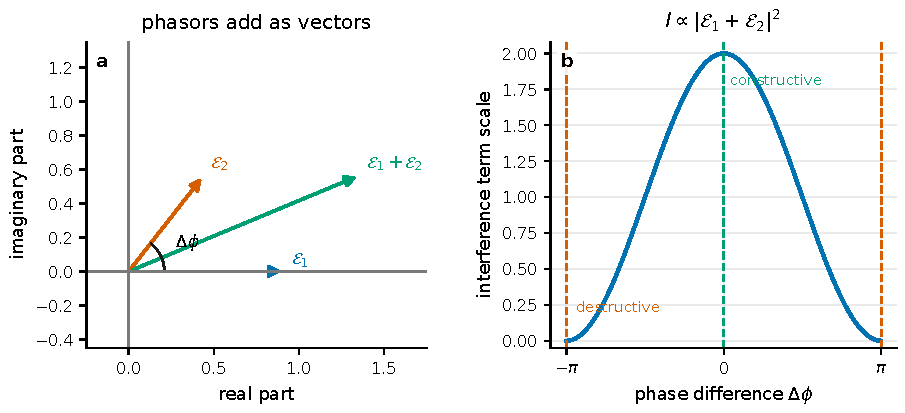
\includegraphics[width=0.85\linewidth]{figures/generated/chapter_01/ch01_phase_interference.pdf}
\caption{复振幅与两束光干涉的基本图像。复振幅是一支箭头，长度是振幅、方向是相位；两束光先做箭头的向量相加，探测器再取合成箭头长度的平方。相位差 \(\Delta\phi\) 决定干涉项是加强（相长）、抵消（相消），还是在相位乱变时被平均掉。}
\label{fig:e01-phase-interference}
\end{figure}

\section{几何相位：路程差是从哪儿来的}
\label{sec:e01-geometry}

上一节的相位差 \(\Delta\phi\) 还很抽象。在天文观测里，它最常见的来源其实非常具体、非常几何：\textbf{两束光走的路不一样长}。这一节就把这个"路程差"一步步变成相位差。

先立画面。设有一颗很远的星，它发出的光到达地面时，波前（同相位的面）几乎是一张平的大纸，沿着源方向 \(\bm s\)（一个指向星的单位矢量）推进。地面上有两台望远镜，位置相差一个\textbf{基线矢量}（baseline）\(\bm B\)——就是从第一台指向第二台的那根矢量，单位是厘米。因为两台望远镜不在垂直于 \(\bm s\) 的同一张波前上，同一个波前要先到达其中一台、再多走一小段才到另一台。这"多走的一小段"，就是路程差。

多走的路有多长？把基线 \(\bm B\) 投影到源方向 \(\bm s\) 上即可。矢量在某方向上的投影长度正是点积，所以路程差是

\[
  \Delta \ell=\bm B\cdot\bm s .
\]

这一步的几何含义要看清：\(\bm B\cdot\bm s=|\bm B|\cos\theta\)，\(\theta\) 是基线与源方向的夹角。若星就在基线正前方（\(\bm B\) 与 \(\bm s\) 平行），投影最长、路程差最大；若星在基线的正上方（\(\bm B\perp\bm s\)），投影为零、两台望远镜到同一波前的路一样长、没有路程差。这跟日常经验一致：斜着照过来的光，两个接收点之间才有先后。

现在把“多走的一段路”换算成“多转的相位”。这里要用到一个到目前为止还没正式点破、但马上就能从第~\ref{sec:e01-wave} 节的图像自己推出来的事实：波在空间里每前进一个\textbf{波长}（wavelength）\(\lambda\)，相位恰好前进 \(2\pi\)（转满一圈）。为什么？回到第~\ref{sec:e01-wave} 节立好的时间图像——电场每过一个周期 \(T\)，瞬时相位就增加 \(\omega T=2\pi\)（这正是“一个周期转满一圈”的定义）。而在同样这段时间 \(T\) 里，以光速 \(c\) 传播的波正好前进一段距离

\[
  \lambda\ \equiv\ cT=\frac{c}{\nu}=\frac{2\pi c}{\omega}.
\]

这段"相位刚好累积满一圈 \(2\pi\)"所对应的空间长度，就是波长。于是"时间上过了一个周期"和"空间上前进了一个波长"是同一件事的两种说法，相位都恰好前进 \(2\pi\)。这样一来，\(\lambda\) 并不是凭空冒出来的新符号：它由第~\ref{sec:e01-wave} 节反复打磨的 \(\nu\)（或 \(\omega\)）通过 \(\lambda=c/\nu\) 直接定出。代入那里的可见光频率 \(\nu\simeq5\times10^{14}\ {\rm Hz}\)，得 \(\lambda=c/\nu\approx(3\times10^{10}\ {\rm cm\,s^{-1}})/(5\times10^{14}\ {\rm Hz})=6\times10^{-5}\ {\rm cm}=0.6\ \mu{\rm m}\)，正是我们熟悉的可见光波长——和第~\ref{sec:e01-wave} 节"光在一飞秒里跑 \(0.3\ \mu{\rm m}\)"的数字也自洽（两飞秒一个周期，正好跑 \(0.6\ \mu{\rm m}\) 一个波长）。

有了这个"一个波长折算 \(2\pi\)"的汇率，路程差就好换算了：既然多走一个 \(\lambda\) 相位就多转 \(2\pi\)，那么多走 \(\Delta\ell\) 这么长，就是多走了 \(\Delta\ell/\lambda\) 个波长，相位前进了 \(\Delta\ell/\lambda\) 圈，也就是 \(2\pi\times(\Delta\ell/\lambda)\) 弧度。把 \(\Delta\ell=\bm B\cdot\bm s\) 代进去：

\begin{equation}
  \Delta\phi=\frac{2\pi}{\lambda}\,\bm B\cdot\bm s .
  \label{eq:e01-geometric-phase}
\end{equation}
\begin{formulaexplain}
\(\Delta\phi\) 是两束光的几何相位差；\(\bm B\) 是两接收点之间的基线矢量；\(\bm s\) 是源方向单位矢量；\(\bm B\cdot\bm s\) 是投影出来的路程差；前面的 \(2\pi/\lambda\) 是"每个波长折算 \(2\pi\) 相位"的换算系数。
\end{formulaexplain}

把每个部件再点一遍，确保单位对得上。\(\bm B\cdot\bm s\) 是长度，单位厘米；\(\lambda\) 也是长度，单位厘米；两者相除得到"走了多少个波长"，是个无量纲的数；再乘 \(2\pi\)（弧度/圈），就得到无量纲但以弧度计的相位差 \(\Delta\phi\)。量纲严丝合缝。那个 \(2\pi/\lambda\) 常被记作波数 \(k=2\pi/\lambda\)，于是也写成 \(\Delta\phi=k\,\bm B\cdot\bm s\)——它的意思始终是“把长度翻译成相位的汇率”。

代入真实数字，感受一下这个相位差有多大。恒星强度干涉的经典装置——Narrabri 恒星强度干涉仪——最大基线约 \(B\simeq188\ {\rm m}\)、工作波长约 \(\lambda\simeq0.44\ \mu{\rm m}\)；今天用 VERITAS、MAGIC 这类切伦科夫望远镜阵列做强度干涉时，基线也在上百米量级。取一组整齐的代表值 \(B\sim100\ {\rm m}=10^{4}\ {\rm cm}\)、\(\lambda\sim0.5\ \mu{\rm m}=5\times10^{-5}\ {\rm cm}\)，当基线几乎正对源方向时，路程差最大可达 \(\Delta\ell\sim B=100\ {\rm m}\)，于是

\[
  \frac{\Delta\ell}{\lambda}\sim\frac{10^{4}\ {\rm cm}}{5\times10^{-5}\ {\rm cm}}=2\times10^{8}\ (\text{个波长}),\qquad
  \Delta\phi=2\pi\,\frac{\Delta\ell}{\lambda}\sim1.3\times10^{9}\ {\rm rad}.
\]

相位差高达十亿弧度、合两亿多整圈！这就点出了干涉测量的一个基本事实：绝对相位差本身是个天文数字，没人真的去数它一共转了多少整圈。真正被测量、被关心的，是当地球自转让基线 \(\bm B\) 相对源方向 \(\bm s\) 缓慢转动、或者源在天上的位置稍有不同时，这个庞大的 \(\Delta\phi\) 又变化了几圈——也就是干涉条纹\emph{移动了多少个周期}。绝对相位是天文数字，条纹的\emph{相对}移动才是可测、可用的信号。

这条式子看着简单，却是干涉测量的整个出发点：把它代回上一节的 \(2E_1E_2\cos(\Delta\phi)\)，望远镜看到的干涉亮暗就直接和基线 \(\bm B\)、源方向 \(\bm s\) 挂上了钩——转动地球（改变 \(\bm B\) 相对 \(\bm s\) 的投影），或者源的位置稍有不同，条纹就会移动。反过来，从条纹怎么移动，就能反推源在天上的精细结构。不过这里我们只搭好最基础的相位语言；两台望远镜之间更完整的空间相干关系，要到第~\ref{chap:e05} 章及其之后才被正式发展起来。

\section{本章要点}
\label{sec:e01-summary}

\begin{itemize}
  \item 单色光的物理本体是飞快摆动的电场 \(E(t)=E_0\cos(\omega t+\phi)\)；可见光周期只有几飞秒，比任何常规探测器快约百万倍，所以逐周期的振荡与相位探测器\textbf{看不见}。
  \item 复振幅 \(\mathcal E=E_0e^{i\phi}\) 是一支旋转箭头：长度 \(|\mathcal E|=E_0\) 是振幅，方向 \(\arg\mathcal E=\phi\) 是相位。取实部 \(E(t)=\operatorname{Re}[\mathcal E e^{i\omega t}]\) 就还原真实电场；箭头记法让"场的相加"变成简单的向量相加。
  \item 强度 \(I\propto\langle E^2\rangle_{\rm det}=\tfrac12|\mathcal E|^2\)。那个 \(1/2\) 来自 \(\cos^2\) 在一个周期上的平均；快速振荡项被抹平，\emph{单束光的绝对相位不被记录}。
  \item 两束光先加电场后平方：\(I\propto|\mathcal E_1+\mathcal E_2|^2=|\mathcal E_1|^2+|\mathcal E_2|^2+2E_1E_2\cos(\phi_1-\phi_2)\)。干涉项只认相位差：\(\Delta\phi=0\) 相长、\(\Delta\phi=\pi\) 相消、相位乱变则被平均掉。干涉是把看不见的相位差翻译成看得见的亮暗。
  \item 天文里最常见的相位差来自几何路程差 \(\Delta\phi=(2\pi/\lambda)\,\bm B\cdot\bm s\)：\(\bm B\cdot\bm s\) 是基线在源方向上的投影程差，\(2\pi/\lambda\) 把长度换成相位。它是空间相干与干涉成像的起点（第~\ref{chap:e05} 章）。
\end{itemize}

\vspace{0.5em}
\noindent\textbf{想一想。}
(1) 两束等强度的光相长干涉时，峰值强度是单束的四倍——那"多出来的能量"从哪里来，又到哪里去了？
(2) 如果把两台望远镜的基线 \(\bm B\) 转到正好垂直于源方向 \(\bm s\)，几何相位差 \(\Delta\phi\) 等于多少？此时干涉条纹会怎样？
(3) 为什么说"绝对相位测不到，但相位差测得到"这两句话并不矛盾？试着只用式~\eqref{eq:e01-intensity} 和式~\eqref{eq:e01-interference} 来回答。
